\section{Foundations of Parallel and Concurrent Computing}
\label{sec:parallel-concurrent}
\paragraph{}

The MAPF problem involves the simultaneous evolution of multiple agents
within a shared environment. As the number of agents increases, both the computational effort
required to compute individual paths and the complexity of coordinating their interactions grow
rapidly. For this reason, many MAPF approaches rely on principles drawn from parallel and
concurrent computing.

For this reason, concepts from parallel and concurrent computing are particularly relevant for
addressing coordination challenges in MAPF.



\subsection{Parallelism and Concurrency}
\paragraph{}

Parallelism and concurrency are closely related but conceptually distinct notions that describe
different aspects of task execution within a computational system.

In this context, parallelism refers to the simultaneous execution of multiple computational tasks,
typically with the objective of improving performance or reducing overall execution time. It
relies on the availability of multiple processing units, such as multi-core processors, and
focuses on exploiting hardware resources to increase computational throughput
\cite{arpaci2018operating}.

Concurrency, in contrast, concerns the logical composition of multiple tasks that make progress overlapping periods of time, regardless of whether they are executed simultaneously in
physical terms. These concepts are visually illustrated in Figure~\ref{fig:par_vs_conc}.

\begin{figure}[H]
    \centering
    \begin{subfigure}{0.40\linewidth}
        \centering
        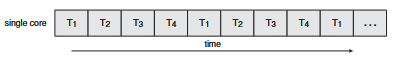
\includegraphics[width=\linewidth]{concurrency.png}
        \caption{Concurrent execution}
    \end{subfigure}
    \hspace{0.02\linewidth}
    \begin{subfigure}{0.35\linewidth}
        \centering
        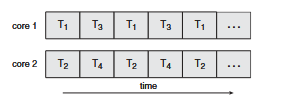
\includegraphics[width=\linewidth]{parallelism.png}
        \caption{Parallel execution}
    \end{subfigure}
    \caption{Conceptual distinction between concurrency and parallelism \cite{silberschatz2018operating}.}
    \label{fig:par_vs_conc}
\end{figure}

\subsection{Computational Models and Execution}
\paragraph{}

Computational models provide an abstract description of how tasks are executed and how
computational resources are organized during execution. These models are essential for reasoning
about the structure, scalability, and coordination of computations involving multiple activities
that progress over time.

\subsubsection{Processes}
\paragraph{}

A process represents an executing instance of a program together with its associated execution
context. This context typically includes a private address space, program code, data, and
operating system resources required for execution \cite{tanenbaum2015modern}.

Processes provide strong isolation between executing programs, as each process operates within
its own protected memory space. This isolation improves robustness and fault containment, since
errors in one process cannot directly corrupt the state of another. However, inter-process
communication generally incurs higher overhead, as it requires explicit mechanisms to exchange
data across process boundaries \cite{silberschatz2018operating}.

From an execution perspective, processes constitute units of concurrency that provide strong
isolation, at the cost of increased management and communication overhead.



\subsubsection{Threads}
\hspace{\parindent}
A thread represents a lower-level unit of execution within a process. Multiple threads within
the same process share the process address space and resources, while maintaining independent
execution contexts such as program counters and stacks \cite{tanenbaum2015modern}. This sharing
enables efficient communication and cooperation between concurrent activities, as data can be
accessed directly without inter-process communication mechanisms.

Threads can be classified according to how their management is implemented. In user-level
threading models, thread creation, scheduling, and synchronization are handled by runtime systems
operating entirely in user space. As depicted in Fig.~\ref{fig:user_kernel_threads}(a), the kernel
is unaware of individual threads and schedules only processes, while thread tables and scheduling
decisions are maintained by the runtime environment. This approach enables fast thread
management but limits the ability to exploit multiple processors transparently
\cite{silberschatz2018operating}.

In contrast, kernel-level threads, shown in Fig.~\ref{fig:user_kernel_threads}(b), are
managed directly by the operating system kernel. In this model, the kernel maintains thread
tables and schedules threads independently, allowing threads belonging to the same process to be
distributed across multiple processing units. While this enables true parallel execution on
multi-core systems, it also introduces higher management overhead due to kernel involvement
\cite{arpaci2018operating}.


\begin{figure}[H]
    \centering
    \begin{subfigure}{0.4\linewidth}
        \centering
        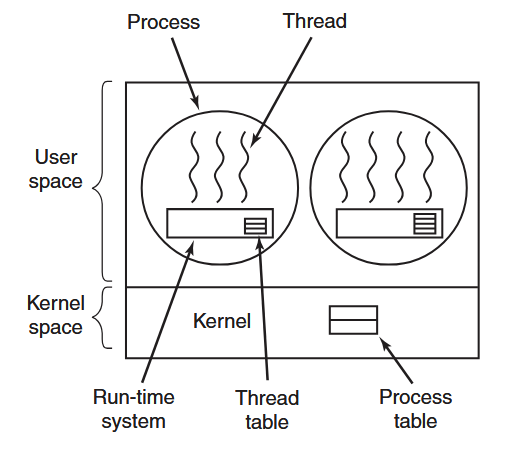
\includegraphics[width=\linewidth]{userthreads.png}
        \caption{User-level threading model}
    \end{subfigure}
    \hspace{0.02\linewidth}
    \begin{subfigure}{0.36\linewidth}
        \centering
        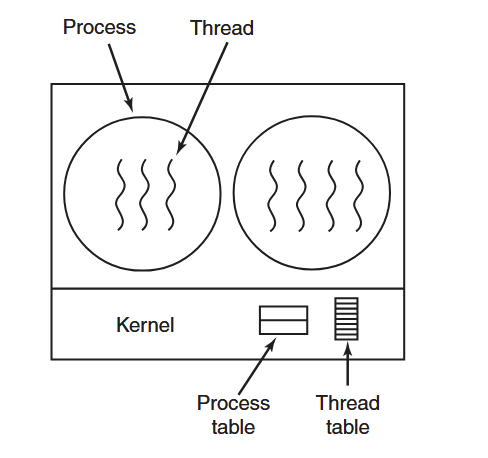
\includegraphics[width=\linewidth]{kernelthreads.png}
        \caption{Kernel-level threading model}
    \end{subfigure}
    \caption{Conceptual comparison between user-level and kernel-level thread management \cite{tanenbaum2015modern}.}
    \label{fig:user_kernel_threads}
\end{figure}

In both models, threads within a process typically share memory and other resources, adopting a
shared-memory execution model. While this model supports efficient cooperation, it also requires
careful coordination to ensure correct access to shared data. The mechanisms used to address
these challenges are discussed in the following subsection.



\subsection{Synchronization and Shared Resource Access}
\hspace{\parindent}
In concurrent execution models, multiple threads or tasks may access shared resources during
their execution. While shared access enables cooperation and efficient communication, it also
introduces challenges related to correctness, as uncontrolled interactions may lead to
inconsistent or unintended system states.

\subsubsection{Race Conditions}
\paragraph{}

In concurrent execution models, incorrect synchronization may result in race
conditions, where the behavior of a computation depends on the timing of concurrent executions. When multiple threads access shared
resources without proper coordination, the final system state may vary across different
execution schedules, even when the same operations are performed \cite{arpaci2018operating}.

Race conditions are particularly difficult to detect and reason about, as they often arise
only under specific execution orders of concurrent tasks.


\subsubsection{Critical Sections}
\paragraph{}

To prevent race conditions, concurrent systems identify regions of execution that access shared
resources as critical sections. A critical section denotes a portion of code in which a
shared resource is accessed or modified and whose execution must be mutually exclusive.

Correct concurrent execution requires that critical sections operating on the same shared
resource are not executed simultaneously by multiple threads, thereby ensuring consistency of
the shared state \cite{tanenbaum2015modern}.


\subsubsection{Mutexes}
\paragraph{}

Mutual exclusion mechanisms, commonly referred to as mutexes, provide a concrete means
to enforce exclusive access to critical sections. A mutex ensures that at most one thread may
enter a given critical section at any time.

By serializing access to shared resources, mutexes prevent concurrent modifications that could
otherwise result in inconsistent system states. This behavior is illustrated in Fig.~\ref{fig:critical}, where one process is blocked while another executes a critical section.


\begin{figure}[H]
    \centering
    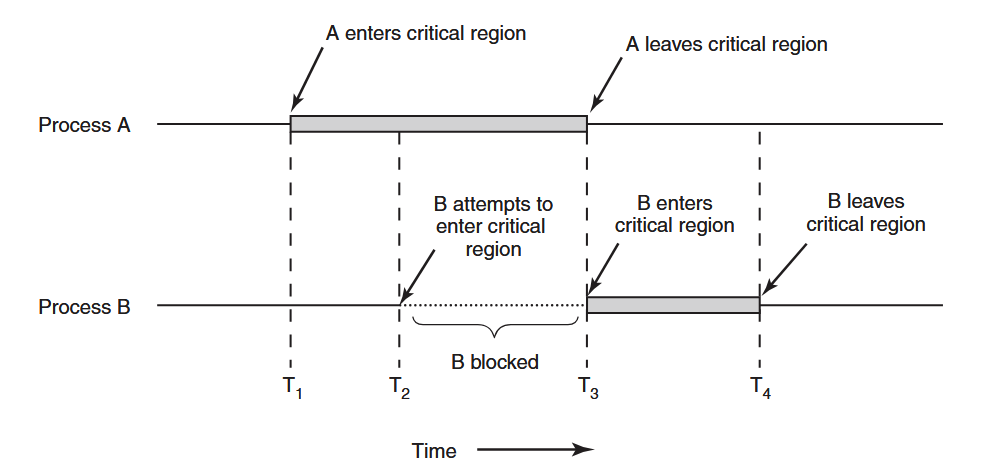
\includegraphics[width=0.8\linewidth]{critical_region.png}
    \caption{Illustration of mutual exclusion in a critical section \cite{tanenbaum2015modern}.}
    \label{fig:critical}
\end{figure}

\subsubsection{Semaphores}
\paragraph{}

Semaphores provide a general synchronization for controlling access to shared resources
and enforcing ordering constraints between concurrent tasks. Unlike mutexes, which are primarily
intended to enforce exclusive access, semaphores support more flexible coordination patterns
\cite{dijkstra1968cooperating}.

According to Arpaci-Dusseau \cite{arpaci2018operating}, semaphores are commonly
classified into two types:
\begin{itemize}
    \item \textbf{Binary semaphores}, whose value is restricted to zero or one, and which can be
    used to enforce mutual exclusion in a manner similar to mutexes, though without ownership
    constraints;
\item \textbf{Counting semaphores}, which take non-negative integer values and are used to
manage access to a finite number of identical resources. The semaphore value represents the
number of currently available resource instances and is decremented each time a resource is
allocated to a process or thread.

\end{itemize}


\subsubsection{Deadlocks}
\paragraph{}

Another fundamental challenge in concurrent systems is deadlock, a state in which a set
of threads becomes permanently blocked because each thread is waiting for resources held by
others. Deadlocks arise from circular waiting dependencies and result in a loss of system
progress, requiring careful design and coordination to avoid
\cite{silberschatz2018operating}.





\section{Summary}
\paragraph{}
This chapter introduced the main background concepts required to support the work developed in this dissertation. First, the MAPF problem was formally defined as the computation of conflict-free trajectories for multiple agents moving in a shared environment, highlighting the role of time, agent interactions, and global optimization criteria. The chapter then discussed how MAPF problems can be represented using discrete environment models, with particular emphasis on grid-based and graph-based abstractions.

Classical graph search methods were also reviewed, since they provide the basis for individual path computation in many multi-agent planning approaches. In particular, Dijkstra's algorithm and A* were introduced as fundamental shortest-path methods, together with their main properties and computational complexity.

The chapter further presented basic machine learning concepts relevant to the proposed heuristic analysis. Clustering methods, namely K-means and DBSCAN, were introduced as tools for characterizing the spatial distribution of robots, while linear regression was presented as an exploratory model for empirical runtime analysis. Finally, concepts from parallel and concurrent computing were discussed, including parallelism, concurrency, processes, threads, synchronization mechanisms, race conditions, critical sections, mutexes, semaphores, and deadlocks.

Overall, these topics establish the theoretical and technical foundation for the multi-robot planning methods, prioritization heuristics, runtime analysis, and parallel execution strategies discussed in the following chapters.